\documentclass[a4paper]{article}
\usepackage{ctex}
%\usepackage[slantfont, boldfont, CJKtextspaces, CJKmathspaces]{xeCJK}
\usepackage{fontspec,xunicode,xltxtra}
\usepackage[pagestyles]{titlesec}
\usepackage{indentfirst}
\usepackage[top=1in,bottom=1in,left=1.25in,right=1.25in]{geometry}
\usepackage{amsmath}
%\usepackage[usenames,dvipsnames]{color}
\usepackage[colorlinks,linkcolor=red,anchorcolor=Blue,citecolor=green]{hyperref}
\usepackage{graphicx}

%\setCJKmainfont[BoldFont={黑体}, ItalicFont={楷体_GB2312}]{宋体}
\setmainfont{Liberation Serif} 
\setsansfont{Liberation Sans} 
\setmonofont{文泉驿等宽微米黑}

%\punctstyle{kaiming} % 开明式标点格式 
\renewcommand{\today}{}

\begin{document}

\title{Maze解题报告}
\author{成都七中\ \  王迪}
\maketitle
\tableofcontents

\newpage

\section{题目大意}
在二维坐标系中给出一个$N$个点的简单直角多边形(不自交,无空洞,每条边都平行于坐标轴),和$M$组询问,每个询问由两个多边形内的点$(X_S,T_S),(X_T,Y_T)$组成,计算$S$点和$T$点间的最短距离:仅可以沿水平方向或竖直方向运动,且不能走出多边形。 \par
有$5\%$的数据,$N=4$; \par
有$20\%$的数据,$N \le 300$,$M \le 50$; \par
有$10\%$的数据,$N \le 5 \times 10^3$,$M \le 10^5$; \par
有$25\%$的数据,$N \le 10^5$,$M \le 300$; \par
对于$100\%$的数据,$N \le 10^5$,$M \le 10^5$,坐标均是不超过$10^8$的非负整数。

\section{基础知识}
这篇题解假定大家对计算几何有基本的了解,知道离散化和扫描线算法,会至少一种平衡树,了解树上的倍增算法。请不了解的同学自行学习。

\section{算法分析}
这道题有着比较浓的计算几何背景,同时多组询问的形式提示我们要使用高效的数据结构进行维护。 \par
对于这类题目我们的常用方法是:先考虑处理一组询问,再考虑加速处理过程。

\section{$5\%$的算法}
注意到有$5\%$的数据$N=4$,由题意知多边形只可能是一个矩形。 \par
所以$S$和$T$之间的最短距离就是它们的曼哈顿距离,即$|X_S-X_T|+|Y_S-Y_T|$。 \par
对于每组询问直接输出即可。时间复杂度$O(M)$,期望得分$5$分。

\section{$25\%$的算法}
有$20\%$的数据$N \le 300, M \le 50$,因为规模较小,我们可以借助一些图论的知识来求最短路。 \par
一个比较直接的想法是,把多边形内所有的整点作为点,相邻的整点间连边,然后通过广度优先搜索求解最短路。但坐标范围很大,导致点的数目很多,故需要优化。 \par
对于计算几何,减少冗余点的有效方法之一就是:离散化。 \par
\begin{center}
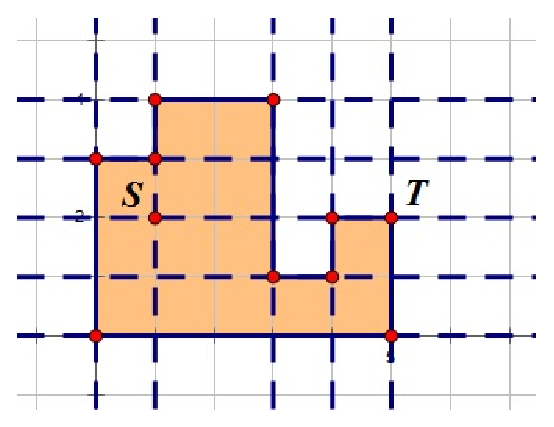
\includegraphics[height=128pt]{maze_0.eps}
\end{center}
\par
如上图,我们把每一条横向边所在直线、纵向边所在直线以及每个询问点所在的横纵直线,都画出来,这样横纵各有$O(N+M)$条直线。容易知道只有这些直线的交点是有用的。 \par
以这些直线的交点为点,每个点向上下左右最近的点连边,这样就变成了一个最短路问题。 \par
若用Dijkstra实现最短路则时间复杂度为$O(M(N+M)^2\log{(N+M)})$,结合之前的算法可以得到$25$分。

\section{$35\%$的算法}
有$10\%$的数据$N \le 5 \times 10^3$,而询问则非常多,对于每组询问单独求最短路复杂度已经无法承受了。 \par
计算几何中常用的思考方法之一:分离横纵坐标。在问题中$X$坐标和$Y$坐标是耦合的,我们可以尝试解耦合,将最短距离分成独立的两个方向。 \par
根据之前用过的曼哈顿距离可猜想:两点间最短距离=连接两点任意路径$X$方向上的最短距离+连接两点任意路径$Y$方向上的最短距离。 \par
可以证明这个猜想是正确的。我们先来考虑算法。 \par
于是我们可以分开考虑$X$和$Y$坐标。以$X$坐标为例,我们用之前提到的离散化把多边形剖成若干个矩形,再把左右边界横坐标相同且位置相邻的矩形合并,如下图:
\begin{center}
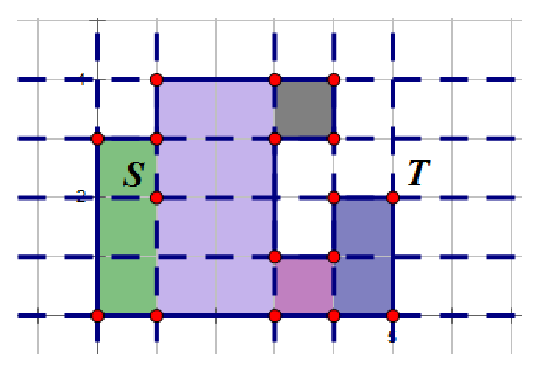
\includegraphics[height=128pt]{maze_1.eps}
\end{center}
\par
我们发现,不同的矩形间构成了一棵树!现在我们来考虑之前提到的猜想,若最短路径在$X$方向上走的不是最短,即在我们的这棵树上不是最短路径,这说明我们在一个矩形内并没有走最短路径,而在矩形中是有最短路径的,所以这条路径不可能最优,反过来说明了我们的猜想正确。 \par
设矩形个数为$T$,于是我们的问题转化成了两个:求出一个点所在的矩形;求树上两个点之间的最短距离。 \par
\subsection{点的定位}
对于第一个问题,由于我们的矩形都是不相交的,且$X$方向上相交的矩形,它们在$X$轴上的投影是相同的!所以可以先对所有矩形排序,然后通过两次二分得到一个点所在的矩形。预处理时间复杂度$O(T\log{T})$,每次点定位复杂度$O(\log{T})$。 \par
\subsection{距离查询}
对于第二个问题,我们可以改造经典的倍增算法:令$dis[j][i][L/R][L/R]$表示从树上$i$号矩形的左边界或右边界,向父亲方向走$2^j$步,走到对应矩形的左边界或右边界,的最短距离。这个可以按$j$划分阶段,用一个简单的动态规划算出。预处理时间复杂度$O(T\log{T})$,每次询问复杂度$O(\log{T})$。 \par
\vspace{15pt}
所以时间复杂度就是$O(T\log{T} + M\log{T})$,注意$X$方向和$Y$方向要分别计算。而$T=O(N^2)$,见下图:
\begin{center}
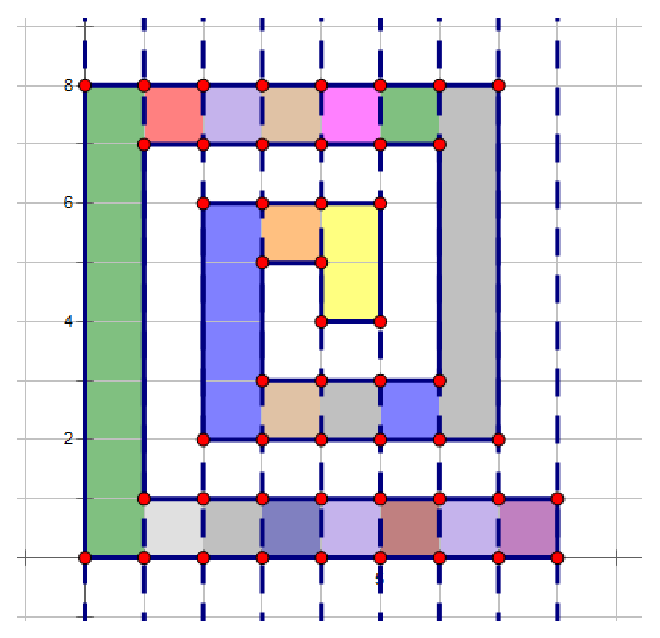
\includegraphics[height=128pt]{maze_2.eps}
\end{center}
\par
结合之前的算法,期望得分$35$到$45$分。

\section{$60\%$的算法}
有$25\%$的数据$N$非常大,而$M$比较小。之前提到的建图方式已经不再适用,我们要寻求一个矩形数目$O(N)$的建图方式。 \par
注意到上面说明$T=O(N^2)$的图中,在某一行上有一些连续的小矩形,而实际处理时我们是可以把它们合并后再考虑的,如下图:
\begin{center}
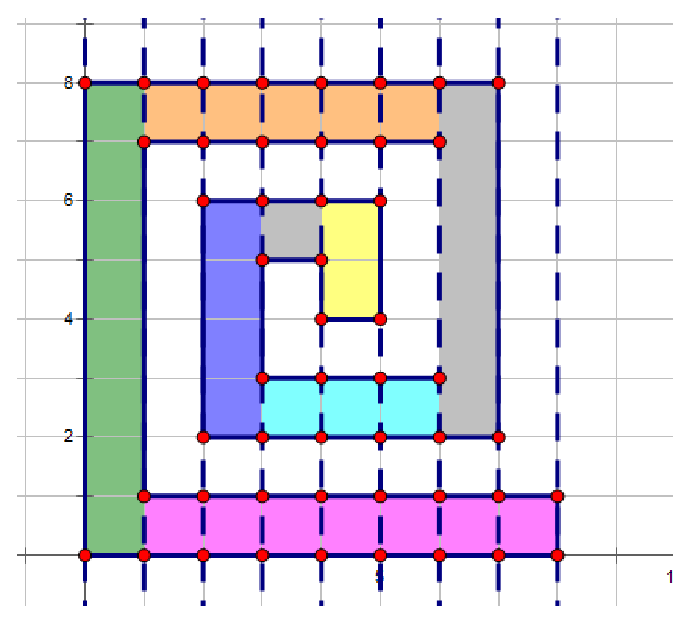
\includegraphics[height=128pt]{maze_3.eps}
\end{center}
\par
此时,矩形数目是$O(N)$的,而且所有矩形仍然构成一棵树。此时我们的问题是:对一个多边形寻找一个$O(N)$的矩形的剖分。 \par
我们需要计算几何中另外一个常用算法:扫描线。 \par
以上图为例,我们取每一条竖直的直线为扫描线,从左到右扫描,维护以当前扫描线为右边界的所有矩形。 \par
那么考虑下一条扫描线对这些矩形的影响。下一条扫描线上有若干不相交的线段,这些线段可能造成的影响有$4$种:
\begin{itemize}
\item “新建”一个矩形;
\item “终止”一个矩形;
\item “分割”一个矩形;
\item “合并”一些矩形。
\end{itemize}
\par
注意到这些情况非常复杂且不好处理,我们需要寻求更有统一性的算法。 \par
而我们维护的,是当前扫描线上的若干矩形,它们在$Y$轴上的投影是一些离散的线段,而我们插入的下一条扫描线,其在$Y$轴上的投影也是一些离散的线段。通过一些计算我们发现,插入扫描线的过程其实是一个异或操作!即:原来的线段和新的线段重叠的部分会“消失”,原来的线段的其他部分会“延续”,新的线段的其他部分则相当于“新建”。这样的话,我们就只需要取出与新扫描线相交的若干线段,取异或后放回,就完成了我们的维护过程。 \par
异或的实现方法就比较简单了,我们只需要将参与异或的线段的端点取出后排序,设排序后的点是$P_0,P_1,\cdots,P_{2k-1}$,那么产生的线段就是$P_{2i}P_{2i+1}$,其中$0\le i <k$。 \par
剩下的问题是,如何高效地维护扫描线上的若干线段。这个可以使用平衡树实现。使用C++的选手可以使用STL的set简化代码。 \par
由上面的分析容易知道,矩形的个数是$O(N)$的,整个矩形剖分的过程是$O(N\log{N})$的,由于询问较少,我们可以通过枚举找到询问点所处的矩形,然后暴力计算答案。 \par
时间复杂度$O(N\log{N}+MN)$。结合之前的算法可以得到$60$到$80$分。

\section{$100\%$的算法}
在上一个算法中,我们的瓶颈在于点定位。其实我们可以在进行矩形剖分时顺便找出每个询问点所处的矩形。 \par
先把所有点按$X$坐标的顺序排序,那么在我们的扫描过程中,当某次扫描线$X=X_0$的$X_0$第一次不小于我们查询点的$X$坐标时,我们可以在平衡树中查询$Y$坐标所属的线段,以确定点所在的矩形。在回答询问时结合之前提到的倍增算法就能得到高效的算法了。 \par
时间复杂度$O((N+M)\log{N})$,期望得分$100$分。

\end{document}
